\documentclass[12pt]{article}
\usepackage{mathptmx}
\usepackage[T1]{fontenc}
\usepackage[latin9]{inputenc}
\usepackage[a4paper, left=2.5cm, right=2.5cm, top=2.5cm, bottom=2.5cm]{geometry}
\geometry{verbose}
\usepackage{booktabs}
\usepackage{amsmath}
\usepackage{amssymb}
\usepackage{graphicx}
\PassOptionsToPackage{version=3}{mhchem}
\usepackage{mhchem}
\usepackage[unicode=true,
bookmarks=false,
breaklinks=false,pdfborder={0 0 1},backref=section,colorlinks=false]
{hyperref}

\makeatletter

\usepackage{times}
\usepackage{xcolor}
\usepackage{setspace}
\usepackage{amsfonts}
\usepackage{tikz}
\usepackage{booktabs}
\usepackage[nottoc,numbib]{tocbibind}

\makeatother

\begin{document}
	%\begin{center}
	%	\onehalfspacing
	%	{\large
	%		Supplementary Information for
	%		\vspace{0.5cm}\\
	%		
	%	\textbf{The Kaposi\textquoteright s sarcoma-associated herpesvirus (KSHV) ORF45 protein promotes the assembly of the active ERK-RSK complex
	%and protects from phosphatases}
	%}\vspace{0.5cm}\\
	%Anita Alexa, Péter Sok, Fridolin Gross, Krisztián Albert, Ádám L.~Póti, Isabel Bento, Andrea Ciliberto, Attila Reményi
	%\vspace{0.5cm}\\
	%\end{center}
	
	{\noindent\Large \textbf{Supplementary Methods}}
	
	\section{Description of the Model}
	The model describes the phosphorylation and dephosphorylation of the kinases ERK and RSK and their interaction with the viral protein ORF45. The architecture of the model captures the binding and catalytic events correctly where docking motif, docking groove, and catalytic site accessibility are taken into account based on mechanistic studies. It consists of a set of ordinary differential equations (ODEs) and is simulated and analyzed using the Python package ``SloppyCell'' and custom written scripts in Python. Two versions of the model are considered, one that describes the SPR experiments and one that describes the \textit{in vitro} and \textit{in cell} experiments. Both are available as SBML files.
	
	The model consists of the three ``basic'' molecular species ERK
	(called \texttt{E} in the model), RSK (\texttt{R}), and ORF45 (\texttt{O}).
	Each of these species can bind to the other two individually, but
	one of the species may also be bound to the two others at the same
	time, thus giving rise to different variants of ternary complexes.
	The three species can also form a ``closed'' complex in
	which each of the species is bound to both of the others.
	
	Apart from engaging in binding reactions, ERK and RSK can also be
	phosphorylated and dephosphorylated. In the model the phosphorylated
	forms are abbreviated as \texttt{pE} and \texttt{pR}, respectively.
	
	Free ERK is phosphorylated by the activated kinase MKK (\texttt{pK} in the model)
	and dephosphorylated by the phosphatase MKP (\texttt{P} in the model). RSK is phosphorylated by phosphorylated ERK. Importantly, RSK can be phosphorylated by ERK only when the latter is not bound to ORF45. RSK is dephosphorylated by a phosphatase that is referred to as \texttt{P2} in the model. RSK can only interact with the phosphatase when it is not directly bound to ORF45.
	
	The kinase MKK also occurs in an inactive form (\texttt{K}).
	Its activation is guided by upstream processes that are not represented
	in detail in the model (see Section~\ref{sss:activation}).
	
	\begin{figure}[h!]
		\centering 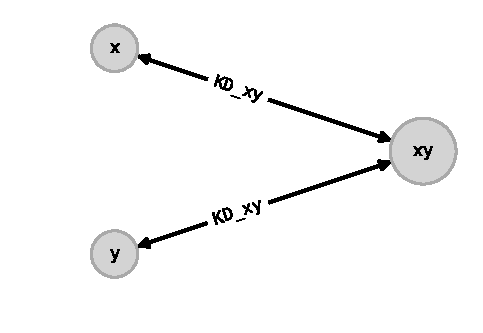
\includegraphics[width=0.5\linewidth]{../res/diagram_reaction_scheme}
		\caption{The reactions occurring in the model are represented using separate
			arrows from the reactants to the product. Double arrows indicate reversible
			reactions.}
		\label{fig:scheme} 
	\end{figure}
	
	
	\section{Terminology}
	
	In order to visualize the model, we use the basic scheme
	that is illustrated in Figure~\ref{fig:scheme}.
	
	All binding reactions and possible complexes are shown in Figure \ref{fig:diagram}. At the center of the diagram are the ``basic'' species (\texttt{O}, \texttt{R}, \texttt{E}, \texttt{pE}, and \texttt{pR}). Binary complexes are denoted by combining the letters corresponding to the respective
	basic species (e.g. \texttt{EpR} for the binary complex consisting
	of ERK and pRSK). For the ternary complexes the names of the species	that directly bind are assembled together to groups, and those groups are then concatenated by underscores. So, for example, \texttt{pEO\_pER} refers to the ternary complex in which pERK is directly bound to both ORF45 and RSK, but ORF45 and RSK do not directly bind each other.
	
	Aside from the individual molecular species, we introduce variables
	that represent the total concentration of each of the molecular species
	and that are referred to as \texttt{Otot}, \texttt{Rtot}, \texttt{Etot},
	\texttt{pRtot}, and \texttt{pEtot}, respectively. They correspond
	to the sum of concentrations of all species in which the corresponding
	combination of letters can be found. So, for example, \texttt{pRtot}
	is the sum of the concentrations of all components that are colored
	either blue or green in the diagram in Figure~\ref{fig:diagram}.
	
	\begin{figure}[h!]
		\centering 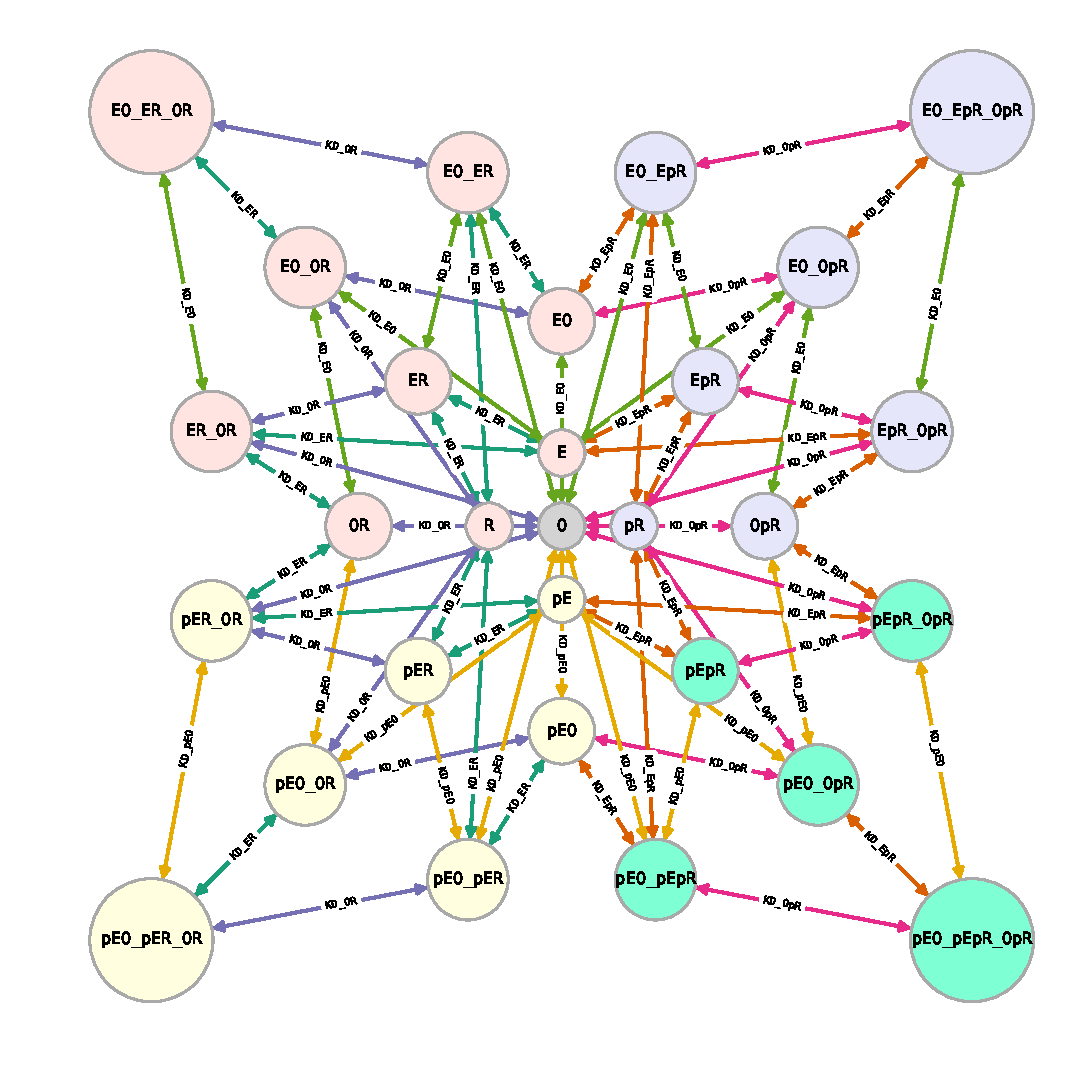
\includegraphics[width=\linewidth]{../res/diagram_all}
		\caption{Diagram showing all binding reactions and the possible complexes formed
			by the three basic components ERK (\texttt{E}), RSK (\texttt{R}),
			and ORF45 (\texttt{O}). The colors are used to group species that
			either include the unphosphorylated forms \texttt{E} and \texttt{R}
			(red), phosphorylated \texttt{pE} and unphosphorylated \texttt{r}
			(yellow), unphosphorylated \texttt{E} and phosphorylated \texttt{pR}
			(blue), or both phosphorylated (green). The colors of the arrows serve
			to highlight reactions with the same dissociation constant.}
		\label{fig:diagram} 
	\end{figure}
	
	\begin{figure}[h!]
		\centering 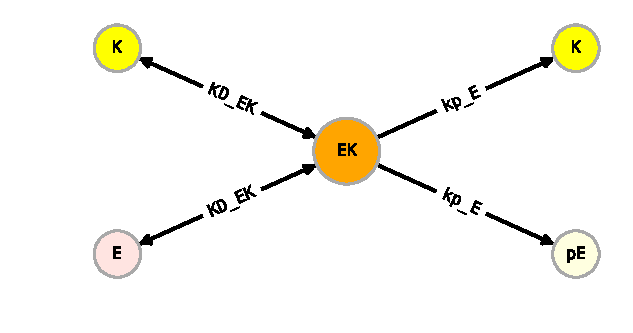
\includegraphics[width=0.45\linewidth]{../res/diagram_EK}
		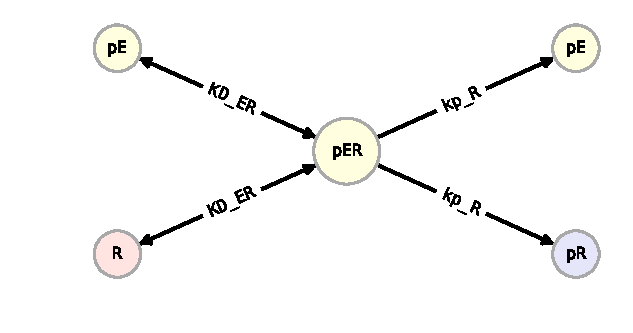
\includegraphics[width=0.45\linewidth]{../res/diagram_pER}\\
		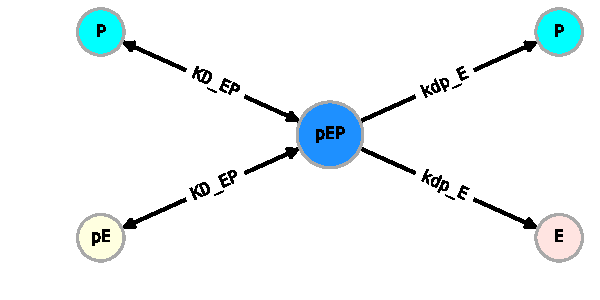
\includegraphics[width=0.45\linewidth]{../res/diagram_EP}
		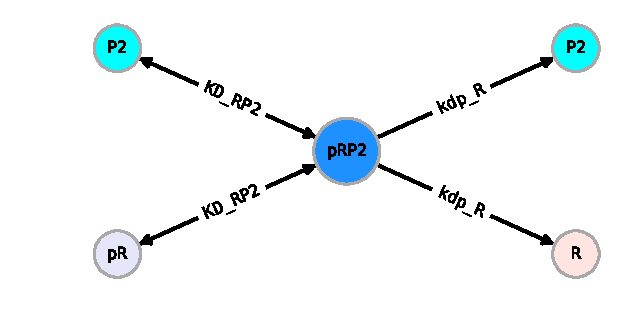
\includegraphics[width=0.45\linewidth]{../res/diagram_RP2}
		\caption{Diagram showing phosphorylation and dephosphorylation in the model.
			Note that binding reactions are reversible (indicated
			by double arrows) and catalytic reactions are irreversible. The figure shows only reactions involving the basic species. For the full list of catalytic reactions see section \ref{s:reactions}.}
		\label{fig:catalytic} 
	\end{figure}
	
	
	\section{Model Equations}
	The full model consists of 34 coupled ODEs. Instead of writing them
	all down explicitly, we provide the general
	form of the equations, which is based on straightforward mass-action
	and Michaelis-Menten kinetics. A full list of all reactions that enter into these equations can be found in Section \ref{s:reactions}.
	
	\subsection{Association and Dissociation Reactions}
	
	All binding and dissociation reactions are reversible and of the form
	\begin{equation}
		s_{i}(\texttt{x})+s_{j}(\texttt{y})\ce{<=>[\texttt{kon\_xy}][\texttt{koff\_xy}]}s_{k}(\texttt{xy})\,,
	\end{equation}
	where $s_{i}(\texttt{x})$ and $s_{j}(\texttt{y})$ refer to the species
	\texttt{x} and \texttt{y} or to complexes containing these species,
	and $s_{k}(\texttt{xy})$ is a complex in which \texttt{x} and \texttt{y}
	are bound. The parameters \texttt{kon\_xy} and \texttt{koff\_xy} are the rates of the forward and reverse reactions, respectively. The corresponding differential equation is of the form 
	\begin{equation}
		\frac{d}{dt}[s_{k}(\texttt{xy})]=\texttt{kon\_xy}\cdot[s_{i}(\texttt{x})]\cdot[s_{j}(\texttt{y})]-\texttt{koff\_xy}\cdot[s_{k}(\texttt{xy})]+\cdots\,.
	\end{equation}
	The square brackets stand for concentrations, and the dots ($\cdots$)
	indicate that there are possible further reactions that contribute
	to the formation, transformation or dissociation of the complex $s_{k}(\texttt{xy})$.
	The dissociation constant is defined in the usual way as 
	\begin{equation}
		\texttt{KD\_xy}=\frac{\texttt{koff\_xy}}{\texttt{kon\_xy}}\,.
	\end{equation}
	
	
	\subsection{Catalytic Reactions}
	
	Phosphorylation reactions are of the form 
	\begin{equation}
		\ce{\texttt{k} + \texttt{s} <=>[\texttt{kon\_ks}][\texttt{koff\_ks}] \texttt{ks} ->[\texttt{kp\_s}] \texttt{k} + \texttt{p}}\,,
	\end{equation}
	where \texttt{k} is the kinase, \texttt{s}
	is the substrate (unphosphorlyated form of a species),
	and \texttt{p} is the product (the phosphorylated form of the same species). The parameter \texttt{kp\_s} is the rate
	of the irreversible catalytic part of the reaction. Dephosphorylation reactions are of analgous form, using the parameter \texttt{kdp\_s} for rate of the catalytic step.
	
	The basic scheme of the catalytic reactions is depicted in Figure~\ref{fig:catalytic}. Note that kinases
	and phosphatases bind to their phosphorylated and unphosphorylated
	substrates with the same rate, but only one of the forms can undergo
	the catalytic step.
	
	\subsection{Activation of the Pathway}
	
	\label{sss:activation} For the activation of MKK (the kinase acting
	upstream of ERK, called \texttt{K} in the model) we use a simplified kinetics of the form 
	\begin{equation}
		\frac{d}{dt}[\texttt{pK}]=(\texttt{kp\_K\_bg}+\texttt{kp\_K\_egf})\cdot[\texttt{K}]-\texttt{kdp\_K}\cdot[\texttt{pK}]\,,\label{eq:kin}
	\end{equation}
	that is, the transition from the the inactive to the active form and
	its reverse are modeled as single reactions. We distinguish, however,
	between the activation by the upstream activation of the EGF-pathway
	(\texttt{kp\_K\_egf}) and a background activation rate (\texttt{kp\_K\_bg})
	in order to account for the experimental observation that there is
	a non-zero equilibrium level of pERK already before the stimulation
	of the pathway.
	
	\subsection{The Closed Complex}
	
	ERK, RSK, and ORF45 can form a closed ternary complex in which each component is directly bound to the two others. The transition between open ternary complexes and closed complexes has different kinetic properties than the corresponding binary reaction. On the one hand, this is because the conformation of the closed complex may have higher stability leading to a slower dissociation of the binding partners.
	On the other hand, association occurs between proteins that belong
	to the same biochemical entity, which makes this reaction different
	from the usual mass action kinetics. We introduce two parameters,
	\texttt{a} and \texttt{d}, to account for these differences in the
	kinetics of association and dissociation, respectively. Figure~\ref{fig:ternary}
	illustrates this idea schematically.
	
	\begin{figure}[h!]
		\centering 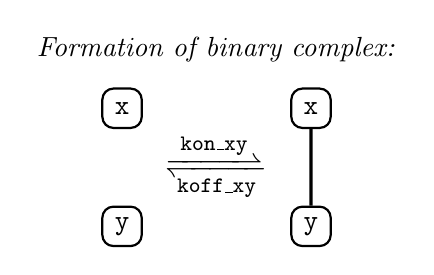
\begin{tikzpicture}[scale=1.5]
			\node at (0.8,1) {\emph{Formation of binary complex:}};
			\node[rectangle,draw, thick, rounded corners, minimum size=0.5cm] (x) at  (0,0.5) {\texttt{x}};
			\node[rectangle,draw, thick, rounded corners, minimum size=0.5cm] (y) at  (0,-0.5) {\texttt{y}};	
			\node (arrows) at (0.8,0) {\large $\ce{<=>[\texttt{kon\_xy}][\texttt{koff\_xy}]}$};
			\node[rectangle,draw, thick, rounded corners, minimum size=0.5cm] (x) at  (1.6,0.5) {\texttt{x}};
			\node[rectangle,draw, thick, rounded corners, minimum size=0.5cm] (y) at  (1.6,-0.5) {\texttt{y}};
			\draw[very thick] (x) -- (y);		
		\end{tikzpicture} \hspace{1.5cm} 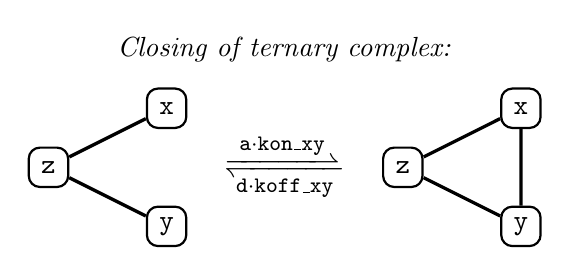
\begin{tikzpicture}[scale=1.5]
			\node at (2,1) {\emph{Closing of ternary complex:}};	
			\node[rectangle,draw, thick, rounded corners, minimum size=0.5cm] (z) at  (0,0) {\texttt{z}};
			\node[rectangle,draw, thick, rounded corners, minimum size=0.5cm] (x) at  (1,0.5) {\texttt{x}};
			\node[rectangle,draw, thick, rounded corners, minimum size=0.5cm] (y) at  (1,-0.5) {\texttt{y}};
			\draw[very thick] (z) -- (x);
			\draw[very thick] (z) -- (y);
			
			\node (arrows) at (2,0) {\large $\ce{<=>[\texttt{a}\cdot\texttt{kon\_xy}][\texttt{d}\cdot\texttt{koff\_xy}]}$};
			
			\node[rectangle,draw, thick, rounded corners, minimum size=0.5cm] (z) at  (3,0) {\texttt{z}};
			\node[rectangle,draw, thick, rounded corners, minimum size=0.5cm] (x) at  (4,0.5) {\texttt{x}};
			\node[rectangle,draw, thick, rounded corners, minimum size=0.5cm] (y) at  (4,-0.5) {\texttt{y}};
			\draw[very thick] (z) -- (x);
			\draw[very thick] (z) -- (y);
			\draw[very thick] (x) -- (y);
		\end{tikzpicture} \caption{Difference in binding kinetics between the formation of a binary complex and the corresponding reaction in the transition from an open to a closed ternary complex. The set of placeholders \texttt{x}, \texttt{y}, and \texttt{z} can be any combination of the basic species (\texttt{E}/\texttt{pE}, \texttt{R}/\texttt{pR}, and \texttt{O}), leading to 8 possibilities of forming a binary and 12 possibilities of closing a ternary complex. While the \texttt{kon\_xy/koff\_xy} can vary depending on the reaction, the factors \texttt{a} and \texttt{d} are assumed to be the same for all reactions.}
		\label{fig:ternary} 
	\end{figure}
	
	The equations that describe the formation of the different closed
	complexes are of the following form:
	
	\begin{equation}
		\frac{d}{dt}[\texttt{cl}]=\texttt{a}\cdot\sum_{i}{\texttt{kon}_{i}}\cdot[\texttt{op}_{i}]-\texttt{d}\cdot\sum_{i}{\texttt{koff}_{i}}\cdot[\texttt{cl}]\,.
	\end{equation}
	Here, \texttt{cl} is one of the four closed complexes (corresponding
	to the four outer vertices in Figure \ref{fig:diagram}). Each of
	these closed complexes can be formed from three different open precursors that are referred to as $\texttt{op}_{i}$. The parameters $\texttt{kon}_{i}$
	and $\texttt{koff}_{i}$ are the association and dissocation rates of the corresponding binary reactions. The parameter \texttt{d} is a dimensionless number that changes each of the binary dissociation
	rates by the same factor. The parameter \texttt{a} has a unit of concentration
	and can be interpreted as the effective concentration that results
	from bringing the binding partners together in the same complex.
	
	\section{Modeling Strategy}
	We determine plausible ranges for those parameters which were not
	directly measured by fitting them to different sets of experimental
	data. We proceed in a step-wise fashion, constraining as many parameters
	as possible with the simpler SPR and \textit{in vitro} experiments
	and fitting only the remaining ones to the \textit{in cell} experiments.
	All parameter values that were used for or obtained from the fitting
	procedures are listed in \textbf{Supplementary Table S2}.
	
	Because SPR, \textit{in vitro}, and \textit{in cell} experiments are
	different in many respects, the parameters were not fixed but they
	were only constrained and were allowed to deviate not much more than
	by $\pm 10\%$ from the determined value. Note though, that these
	constraints are not strict, but that deviations add to the overall
	cost function used for the optimization (For details see the documentation
	of SloppyCell).
	
	In the main figures we only show the simulations corresponding to the best fit. However, SloppyCell allows for an exhaustive search of the parameter space to generate all parameter sets that are statistically consistent with the data. This is particularly important for so-called ``sloppy'' models in which many parameters are poorly constrained. As we show, however, the parameters in our model are reasonably well-constrained, and the model predictions still hold even if based on an ensemble fit (Supplementary Figure 7).
	
	\subsection{SPR Experiments}
	We use the SPR data to obtain the dissociation rates for the binary
	reactions between ppERK, RSK, and ORF45. In addition, the experiment
	including all three species allows us to estimate the parameters \texttt{a}
	and \texttt{d} which describe the behavior of the closed ternary complex.
	
	In SPR experiments a protein of interest (the ligand) is stably bound
	to a surface and can associate with molecules (the analyte) within
	a solution that flows along the surface. Therefore, the concentration of the free analyte stays constant in the association phase. Thus, for the analytes in our experiments (ppERK and ORF45), we have
	the following conservation relations: 
	\begin{align}
		& [\texttt{pE}]=\texttt{pEtot}-\sum_{i}[s_{i}(\texttt{pE})]=\text{const.}\\
		& [\texttt{O}]=\texttt{Otot}-\sum_{i}[s_{i}(\texttt{O})]=\text{const.}\,,
	\end{align}
	where, as before, the $s_{i}(\texttt{E})$, $s_{i}(\texttt{pE})$
	and $s_{i}(\texttt{o})$ denote all the possible complexes that include
	\texttt{E} and \texttt{O}, respectively.
	
	For the ligands (RSK and ORF45\footnote{Note that ORF45 appears both as ligand and as analyte in different
		experiments.}), by contrast, the total amount is constant, leading to the following
	conservation relation: 
	\begin{align}
		& \texttt{Rtot}=[\texttt{R}]+\sum_{i}[s_{i}(\texttt{R})]=\text{const.}\\
		& \texttt{Otot}=[\texttt{O}]+\sum_{i}[s_{i}(\texttt{O})]=\text{const.}
	\end{align}
	
	Another peculiarity of the SPR experiments is that it measures
	the mass of the complexes and not their concentrations. In order to compare the simulations to the data from the experiments involving two analytes we therefore need to take into account the relative weight of the different proteins. For this purpose we introduce a new variable 
	\begin{equation}
		\texttt{Rcomp}=\texttt{E\_weight}\cdot\sum_{i}[s_{i}(\texttt{ER})]+\texttt{O\_weight}\cdot\sum_{i}[s_{i}(\texttt{OR})]\,,
	\end{equation}
	where \texttt{E\_weight} and \texttt{O\_weight} denote the relative
	molecular weights of ERK and ORF45, and the $s_{i}(\texttt{ER})$
	and $s_{i}(\texttt{OR})$ denote all the complexes with RSK in which
	ERK and ORF45 occur, respectively. For all our simulations we chose
	\begin{equation}
		\texttt{O\_weight}=1\quad\text{and}\quad\texttt{E\_weight}=6.3\,,
	\end{equation}
	in agreement with a molecular weight of 6541Da for ORF45 and 41389Da
	for ERK2. The absolute weights are not important for the modeling
	because the data are given in arbitrary units, and we allow for a
	scaling factor that converts model units into the experimental units.
	This scaling factor is optimized along with the parameter fit. For
	the same reason, the absolute amount of ligand bound to the surface
	does not matter for the modeling results. We choose $\texttt{Rtot}=1\mu M$
	and $\texttt{Otot}=1\mu M$ in the respective experiments.
	
	The model is fit to both the association and the dissociation phase
	of the experiments. We model the dissociation phase by setting the
	relevant association rates to zero. All parameters obtained in the fit can be found in Supplementary Table S2.
	
	\subsubsection{RSK and ppERK}
	\label{sss:er} In this case RSK is the ligand, and ppERK is the analyte.
	We use a previously measured value of $\texttt{KD\_ER}=2.5\mu M$ (see Supplementary Figure S4A and S5A). We fit the model to two experiments with different analyte concentrations of $[\texttt{pE}]=0.12\mu M$ and
	$[\texttt{pE}]=1.11\mu M$.
	
	
	\subsubsection{RSK and ORF45}
	In this case RSK is the ligand, and ORF45 is the analyte. We use a
	previously measured value of $\texttt{KD\_OR}=0.0012\mu M$ (Supplementary Figure S4A and S5B). We fit the model to two experiments with two different analyte concentrations of $[\texttt{O}]=0.0005\mu M$ and $[\texttt{O}]=0.0135\mu M$.
	
	
	\subsubsection{ppERK and ORF45}
	
	\label{sss:eo} In this case ORF45 is the ligand, and ppERK is the
	analyte. We use a previously measured value of $\texttt{KD\_pEO}=0.8\mu M$
	(see Figure 2A and Supplementary Figure S5C). We fit the model to one experiment with $[\texttt{pE}]=1.66\mu M$.
	
	
	\subsubsection{RSK, ppERK, and ORF45}
	
	We use the experiment with all three species to obtain values for
	the parameters \texttt{a} and \texttt{d}, which determine the association
	and dissociation rates for the closed complex. In this case RSK is
	the ligand, and we have two analytes, ppERK and ORF45 (see Supplementary Figure S5D). We use the previously measured values of $\texttt{KD\_pEO}=0.8\mu M$ and $\texttt{KD\_OR}=0.0012\mu M$, and $\texttt{KD\_ER}=2.5\mu M$, as well as the values for $\texttt{koff\_ER}$, $\texttt{koff\_OR}$, and $\texttt{koff\_pEO}$ from fitting experiments \ref{sss:er}-\ref{sss:eo}.
	
	We fit the model to two experiments with two different conentrations
	for ppERK, $[\texttt{pE}]=0.12\mu M$ and $[\texttt{pE}]=1.11\mu M$.
	The concentration of ORF45 is in both cases $[\texttt{O}]=10\mu M$.
	
	\subsection{\textit{in vitro} Experiments}
	
	The \textit{in vitro} experiments are used to obtain estimates for
	the parameters related to phosphorylation and dephosphorylation and
	to see whether parameters obtained in the SPR experiments are consistent.
	We constrain those parameters that were previously determined by measurements
	or by fitting the SPR experiments and leave the remaining ones free.
	
	Differently from the SPR experiments, all total species amounts are
	constant throughout the experiments. Therefore, we have conservation
	relations of the form 
	\begin{equation}
		\texttt{xtot}=[\texttt{x}]+\sum_{i}[s_{i}(\texttt{x})]=\text{const.}
	\end{equation}
	for all species \texttt{x}, where \texttt{xtot} denotes the total
	amount, {[}\texttt{x}{]} the concentration of free \texttt{x}, and
	the $[s_{i}(\texttt{x})]$ the concentrations of the different possible
	complexes in which \texttt{x} appears.
	
	In line with the experimental setup, we allow all binding reactions
	to have reached an equilibrium when the experimental intervention
	starts. For this purpose, we run the simulation for $t=1000\min$
	before making the parameter changes that correspond to the intervention.
	
	\paragraph{Experiment 1: MKK, ERK, RSK, $\pm$ ORF45}
	
	In this experiment MKK, (unphosphorylated) ERK, and RSK are mixed
	together with or without ORF45 (Figure 5A). The initiation of kinase
	activity is modeled by setting the parameters \texttt{kcatkin} and
	\texttt{kcatrp}, which determine the phosphorylation of ERK and RSK,
	respectively, from zero to a positive value at $t=1000\min$. In line
	with the experiment, the initial concentrations are: 
	\begin{center}
		\begin{tabular}{ll}
			species  & value ($\mu M$)\\
			\midrule 
			\texttt{Etot}  & 2.0\\
			\texttt{pE}  & 0.0 \\
			\texttt{Ktot}  & 0.25\\
			\texttt{Rtot}  & 2.0 \\
			\texttt{Otot}  & 0.0 or 50.0\\
		\end{tabular}
		\par\end{center}
	
	\paragraph{Experiment 2: ppERK, MKP, $\pm$RSK, $\pm$ORF45}
	
	In this experiment (phosphorylated) ppERK is mixed with MKP in the
	presence or absence of RSK and ORF45 (Figure 5C). The initiation of
	phosphatase activity is modeled by setting the parameter \texttt{Ptot},
	corresponding to the total amount of MKP, from zero to $1\mu M$ at
	$t=1000\min$. In line with the experiment, the initial conditions
	are: 
	\begin{center}
		\begin{tabular}{ll}
			species  & value ($\mu M$)\\
			\midrule 
			\texttt{Etot}  & 1.0\\
			\texttt{pE}  & 1.0\\
			\texttt{Ptot}  & $0\rightarrow1$\\
			\texttt{Rtot}  & 0.0 or 1.0\\
			\texttt{Otot}  & 0.0 or 5.0\\
		\end{tabular}
		\par\end{center}
	
	The optimal parameters resulting from fitting the \emph{in vitro}
	experiments can be found in Supplementary Table S2. Figure 6B of the
	main text shows a visual comparison of data and model simulations.
	
	\subsection{\textit{in cell} Experiments}
	
	\label{ss:incell} We assume that the \textit{in cell} and the \textit{in
		vitro} experiments can be modeled in a similar way. That is, we assume
	that all species are well-mixed and conserved. Additionally, we now
	also introduce a phosphatase acting on RSK (called \texttt{P2}),
	and we include the activation reaction of MKK (\texttt{K}) as described
	in Equation \eqref{eq:kin}. As in the \textit{in vitro} experiments,
	we allow the system to find an equilibrium, but then the stimulus
	is simulated by setting the parameter \texttt{kp\_K\_egf}
	from zero to a positive value. The initial concentrations are 
	\begin{center}
		\begin{tabular}{ll}
			species  & value ($\mu M$)\\
			\midrule 
			\texttt{Ktot}  & 1.2\\
			\texttt{K}  & 1.2 \\
			\texttt{Etot}  & 0.7\\
			\texttt{Rtot}  & 2.0\\			
			\texttt{Otot}  & 1.0\\
			\texttt{Ptot}  & 1.0\\
			\texttt{P2tot}  & 1.0\\
		\end{tabular}
		\par\end{center}
	
	The optimal parameters resulting from fitting the \emph{in cell} experiments can be found in Supplementary Table S2. Figure 6C of the main text shows a visual comparison of data and model simulations.
	
	\subsection{Model Predictions}
	
	The model predictions were obtained by simulating the model in the
	same way as in \ref{ss:incell}, using the optimal \emph{in cell}
	parameter set, except for the indicated changes (see Figure 6D).
	
	\section{Full List of Model Reactions}
	\label{s:reactions}
	\begin{footnotesize}
		\subsection*{ERK RSK binding}
		\begin{tabular}{ll}
\textbf{Reaction} & \textbf{Rate law} \\
\midrule
$ \texttt{E}  +  \texttt{R}  \leftrightharpoons  \texttt{ER}  $ & $ \texttt{kon\_ER}  \cdot  \texttt{[E]}  \cdot  \texttt{[R]}  -  \texttt{koff\_ER}  \cdot  \texttt{[ER]}  $ \\
$ \texttt{pE}  +  \texttt{R}  \leftrightharpoons  \texttt{pER}  $ & $ \texttt{kon\_ER}  \cdot  \texttt{[pE]}  \cdot  \texttt{[R]}  -  \texttt{koff\_ER}  \cdot  \texttt{[pER]}  $ \\
$ \texttt{EO}  +  \texttt{R}  \leftrightharpoons  \texttt{EO\_ER}  $ & $ \texttt{kon\_ER}  \cdot  \texttt{[EO]}  \cdot  \texttt{[R]}  -  \texttt{koff\_ER}  \cdot  \texttt{[EO\_ER]}  $ \\
$ \texttt{E}  +  \texttt{OR}  \leftrightharpoons  \texttt{ER\_OR}  $ & $ \texttt{kon\_ER}  \cdot  \texttt{[E]}  \cdot  \texttt{[OR]}  -  \texttt{koff\_ER}  \cdot  \texttt{[ER\_OR]}  $ \\
$ \texttt{pEO}  +  \texttt{R}  \leftrightharpoons  \texttt{pEO\_pER}  $ & $ \texttt{kon\_ER}  \cdot  \texttt{[pEO]}  \cdot  \texttt{[R]}  -  \texttt{koff\_ER}  \cdot  \texttt{[pEO\_pER]}  $ \\
$ \texttt{pE}  +  \texttt{OR}  \leftrightharpoons  \texttt{pER\_OR}  $ & $ \texttt{kon\_ER}  \cdot  \texttt{[pE]}  \cdot  \texttt{[OR]}  -  \texttt{koff\_ER}  \cdot  \texttt{[pER\_OR]}  $ \\
$ \texttt{EO\_OR}  \leftrightharpoons  \texttt{EO\_ER\_OR}  $ & $\texttt{a} \cdot  \texttt{kon\_ER}  \cdot  \texttt{[EO\_OR]}  - \texttt{d} \cdot  \texttt{koff\_ER}  \cdot  \texttt{[EO\_ER\_OR]}  $ \\
$ \texttt{pEO\_OR}  \leftrightharpoons  \texttt{pEO\_pER\_OR}  $ & $\texttt{a} \cdot  \texttt{kon\_ER}  \cdot  \texttt{[pEO\_OR]}  - \texttt{d} \cdot  \texttt{koff\_ER}  \cdot  \texttt{[pEO\_pER\_OR]}  $ \\
$ \texttt{E}  +  \texttt{RP2}  \leftrightharpoons  \texttt{ERP2}  $ & $ \texttt{kon\_ER}  \cdot  \texttt{[E]}  \cdot  \texttt{[RP2]}  -  \texttt{koff\_ER}  \cdot  \texttt{[ERP2]}  $ \\
$ \texttt{pE}  +  \texttt{RP2}  \leftrightharpoons  \texttt{pERP2}  $ & $ \texttt{kon\_ER}  \cdot  \texttt{[pE]}  \cdot  \texttt{[RP2]}  -  \texttt{koff\_ER}  \cdot  \texttt{[pERP2]}  $ \\
$ \texttt{EO}  +  \texttt{RP2}  \leftrightharpoons  \texttt{EO\_ERP2}  $ & $ \texttt{kon\_ER}  \cdot  \texttt{[EO]}  \cdot  \texttt{[RP2]}  -  \texttt{koff\_ER}  \cdot  \texttt{[EO\_ERP2]}  $ \\
$ \texttt{pEO}  +  \texttt{RP2}  \leftrightharpoons  \texttt{pEO\_pERP2}  $ & $ \texttt{kon\_ER}  \cdot  \texttt{[pEO]}  \cdot  \texttt{[RP2]}  -  \texttt{koff\_ER}  \cdot  \texttt{[pEO\_pERP2]}  $ \\
\end{tabular}
		\subsection*{ERK ORF binding}
		\begin{tabular}{ll}
\textbf{Reaction} & \textbf{Rate law} \\
\midrule
$ \texttt{E}  +  \texttt{O}  \leftrightharpoons  \texttt{EO}  $ & $ \texttt{kon\_EO}  \cdot  \texttt{[E]}  \cdot  \texttt{[O]}  -  \texttt{koff\_EO}  \cdot  \texttt{[EO]}  $ \\
$ \texttt{E}  +  \texttt{OR}  \leftrightharpoons  \texttt{EO\_OR}  $ & $ \texttt{kon\_EO}  \cdot  \texttt{[E]}  \cdot  \texttt{[OR]}  -  \texttt{koff\_EO}  \cdot  \texttt{[EO\_OR]}  $ \\
$ \texttt{ER}  +  \texttt{O}  \leftrightharpoons  \texttt{EO\_ER}  $ & $ \texttt{kon\_EO}  \cdot  \texttt{[ER]}  \cdot  \texttt{[O]}  -  \texttt{koff\_EO}  \cdot  \texttt{[EO\_ER]}  $ \\
$ \texttt{E}  +  \texttt{OpR}  \leftrightharpoons  \texttt{EO\_OpR}  $ & $ \texttt{kon\_EO}  \cdot  \texttt{[E]}  \cdot  \texttt{[OpR]}  -  \texttt{koff\_EO}  \cdot  \texttt{[EO\_OpR]}  $ \\
$ \texttt{EpR}  +  \texttt{O}  \leftrightharpoons  \texttt{EO\_EpR}  $ & $ \texttt{kon\_EO}  \cdot  \texttt{[EpR]}  \cdot  \texttt{[O]}  -  \texttt{koff\_EO}  \cdot  \texttt{[EO\_EpR]}  $ \\
$ \texttt{ER\_OR}  \leftrightharpoons  \texttt{EO\_ER\_OR}  $ & $\texttt{a} \cdot  \texttt{kon\_EO}  \cdot  \texttt{[ER\_OR]}  - \texttt{d} \cdot  \texttt{koff\_EO}  \cdot  \texttt{[EO\_ER\_OR]}  $ \\
$ \texttt{EpR\_OpR}  \leftrightharpoons  \texttt{EO\_EpR\_OpR}  $ & $\texttt{a} \cdot  \texttt{kon\_EO}  \cdot  \texttt{[EpR\_OpR]}  - \texttt{d} \cdot  \texttt{koff\_EO}  \cdot  \texttt{[EO\_EpR\_OpR]}  $ \\
$ \texttt{ERP2}  +  \texttt{O}  \leftrightharpoons  \texttt{EO\_ERP2}  $ & $ \texttt{kon\_EO}  \cdot  \texttt{[ERP2]}  \cdot  \texttt{[O]}  -  \texttt{koff\_EO}  \cdot  \texttt{[EO\_ERP2]}  $ \\
$ \texttt{EpRP2}  +  \texttt{O}  \leftrightharpoons  \texttt{EO\_EpRP2}  $ & $ \texttt{kon\_EO}  \cdot  \texttt{[EpRP2]}  \cdot  \texttt{[O]}  -  \texttt{koff\_EO}  \cdot  \texttt{[EO\_EpRP2]}  $ \\
$ \texttt{EP}  +  \texttt{O}  \leftrightharpoons  \texttt{EPO}  $ & $ \texttt{kon\_EO}  \cdot  \texttt{[EP]}  \cdot  \texttt{[O]}  -  \texttt{koff\_EO}  \cdot  \texttt{[EPO]}  $ \\
$ \texttt{EP}  +  \texttt{OR}  \leftrightharpoons  \texttt{EPO\_OR}  $ & $ \texttt{kon\_EO}  \cdot  \texttt{[EP]}  \cdot  \texttt{[OR]}  -  \texttt{koff\_EO}  \cdot  \texttt{[EPO\_OR]}  $ \\
$ \texttt{EP}  +  \texttt{OpR}  \leftrightharpoons  \texttt{EPO\_OpR}  $ & $ \texttt{kon\_EO}  \cdot  \texttt{[EP]}  \cdot  \texttt{[OpR]}  -  \texttt{koff\_EO}  \cdot  \texttt{[EPO\_OpR]}  $ \\
$ \texttt{EpK}  +  \texttt{O}  \leftrightharpoons  \texttt{EpKO}  $ & $ \texttt{kon\_EO}  \cdot  \texttt{[EpK]}  \cdot  \texttt{[O]}  -  \texttt{koff\_EO}  \cdot  \texttt{[EpKO]}  $ \\
$ \texttt{EpK}  +  \texttt{OR}  \leftrightharpoons  \texttt{EpKO\_OR}  $ & $ \texttt{kon\_EO}  \cdot  \texttt{[EpK]}  \cdot  \texttt{[OR]}  -  \texttt{koff\_EO}  \cdot  \texttt{[EpKO\_OR]}  $ \\
$ \texttt{EpK}  +  \texttt{OpR}  \leftrightharpoons  \texttt{EpKO\_OpR}  $ & $ \texttt{kon\_EO}  \cdot  \texttt{[EpK]}  \cdot  \texttt{[OpR]}  -  \texttt{koff\_EO}  \cdot  \texttt{[EpKO\_OpR]}  $ \\
$ \texttt{EK}  +  \texttt{O}  \leftrightharpoons  \texttt{EKO}  $ & $ \texttt{kon\_EO}  \cdot  \texttt{[EK]}  \cdot  \texttt{[O]}  -  \texttt{koff\_EO}  \cdot  \texttt{[EKO]}  $ \\
$ \texttt{EK}  +  \texttt{OR}  \leftrightharpoons  \texttt{EKO\_OR}  $ & $ \texttt{kon\_EO}  \cdot  \texttt{[EK]}  \cdot  \texttt{[OR]}  -  \texttt{koff\_EO}  \cdot  \texttt{[EKO\_OR]}  $ \\
$ \texttt{EK}  +  \texttt{OpR}  \leftrightharpoons  \texttt{EKO\_OpR}  $ & $ \texttt{kon\_EO}  \cdot  \texttt{[EK]}  \cdot  \texttt{[OpR]}  -  \texttt{koff\_EO}  \cdot  \texttt{[EKO\_OpR]}  $ \\
\end{tabular}
		\subsection*{ppERK ORF binding}
		\begin{tabular}{ll}
\textbf{Reaction} & \textbf{Rate law} \\
\midrule
$ \texttt{pE}  +  \texttt{O}  \leftrightharpoons  \texttt{pEO}  $ & $ \texttt{kon\_EO}  \cdot  \texttt{[pE]}  \cdot  \texttt{[O]}  -  \texttt{koff\_pEO}  \cdot  \texttt{[pEO]}  $ \\
$ \texttt{pE}  +  \texttt{OR}  \leftrightharpoons  \texttt{pEO\_OR}  $ & $ \texttt{kon\_EO}  \cdot  \texttt{[pE]}  \cdot  \texttt{[OR]}  -  \texttt{koff\_pEO}  \cdot  \texttt{[pEO\_OR]}  $ \\
$ \texttt{pER}  +  \texttt{O}  \leftrightharpoons  \texttt{pEO\_pER}  $ & $ \texttt{kon\_EO}  \cdot  \texttt{[pER]}  \cdot  \texttt{[O]}  -  \texttt{koff\_pEO}  \cdot  \texttt{[pEO\_pER]}  $ \\
$ \texttt{pE}  +  \texttt{OpR}  \leftrightharpoons  \texttt{pEO\_OpR}  $ & $ \texttt{kon\_EO}  \cdot  \texttt{[pE]}  \cdot  \texttt{[OpR]}  -  \texttt{koff\_pEO}  \cdot  \texttt{[pEO\_OpR]}  $ \\
$ \texttt{pEpR}  +  \texttt{O}  \leftrightharpoons  \texttt{pEO\_pEpR}  $ & $ \texttt{kon\_EO}  \cdot  \texttt{[pEpR]}  \cdot  \texttt{[O]}  -  \texttt{koff\_pEO}  \cdot  \texttt{[pEO\_pEpR]}  $ \\
$ \texttt{pER\_OR}  \leftrightharpoons  \texttt{pEO\_pER\_OR}  $ & $\texttt{a} \cdot  \texttt{kon\_EO}  \cdot  \texttt{[pER\_OR]}  - \texttt{d} \cdot  \texttt{koff\_pEO}  \cdot  \texttt{[pEO\_pER\_OR]}  $ \\
$ \texttt{pEpR\_OpR}  \leftrightharpoons  \texttt{pEO\_pEpR\_OpR}  $ & $\texttt{a} \cdot  \texttt{kon\_EO}  \cdot  \texttt{[pEpR\_OpR]}  - \texttt{d} \cdot  \texttt{koff\_pEO}  \cdot  \texttt{[pEO\_pEpR\_OpR]}  $ \\
$ \texttt{pERP2}  +  \texttt{O}  \leftrightharpoons  \texttt{pEO\_pERP2}  $ & $ \texttt{kon\_EO}  \cdot  \texttt{[pERP2]}  \cdot  \texttt{[O]}  -  \texttt{koff\_pEO}  \cdot  \texttt{[pEO\_pERP2]}  $ \\
$ \texttt{pEpRP2}  +  \texttt{O}  \leftrightharpoons  \texttt{pEO\_pEpRP2}  $ & $ \texttt{kon\_EO}  \cdot  \texttt{[pEpRP2]}  \cdot  \texttt{[O]}  -  \texttt{koff\_pEO}  \cdot  \texttt{[pEO\_pEpRP2]}  $ \\
$ \texttt{pEP}  +  \texttt{O}  \leftrightharpoons  \texttt{pEPO}  $ & $ \texttt{kon\_EO}  \cdot  \texttt{[pEP]}  \cdot  \texttt{[O]}  -  \texttt{koff\_pEO}  \cdot  \texttt{[pEPO]}  $ \\
$ \texttt{pEP}  +  \texttt{OR}  \leftrightharpoons  \texttt{pEPO\_OR}  $ & $ \texttt{kon\_EO}  \cdot  \texttt{[pEP]}  \cdot  \texttt{[OR]}  -  \texttt{koff\_pEO}  \cdot  \texttt{[pEPO\_OR]}  $ \\
$ \texttt{pEP}  +  \texttt{OpR}  \leftrightharpoons  \texttt{pEPO\_OpR}  $ & $ \texttt{kon\_EO}  \cdot  \texttt{[pEP]}  \cdot  \texttt{[OpR]}  -  \texttt{koff\_pEO}  \cdot  \texttt{[pEPO\_OpR]}  $ \\
$ \texttt{pEpK}  +  \texttt{O}  \leftrightharpoons  \texttt{pEpKO}  $ & $ \texttt{kon\_EO}  \cdot  \texttt{[pEpK]}  \cdot  \texttt{[O]}  -  \texttt{koff\_pEO}  \cdot  \texttt{[pEpKO]}  $ \\
$ \texttt{pEpK}  +  \texttt{OR}  \leftrightharpoons  \texttt{pEpKO\_OR}  $ & $ \texttt{kon\_EO}  \cdot  \texttt{[pEpK]}  \cdot  \texttt{[OR]}  -  \texttt{koff\_pEO}  \cdot  \texttt{[pEpKO\_OR]}  $ \\
$ \texttt{pEpK}  +  \texttt{OpR}  \leftrightharpoons  \texttt{pEpKO\_OpR}  $ & $ \texttt{kon\_EO}  \cdot  \texttt{[pEpK]}  \cdot  \texttt{[OpR]}  -  \texttt{koff\_pEO}  \cdot  \texttt{[pEpKO\_OpR]}  $ \\
$ \texttt{pEK}  +  \texttt{O}  \leftrightharpoons  \texttt{pEKO}  $ & $ \texttt{kon\_EO}  \cdot  \texttt{[pEK]}  \cdot  \texttt{[O]}  -  \texttt{koff\_pEO}  \cdot  \texttt{[pEKO]}  $ \\
$ \texttt{pEK}  +  \texttt{OR}  \leftrightharpoons  \texttt{pEKO\_OR}  $ & $ \texttt{kon\_EO}  \cdot  \texttt{[pEK]}  \cdot  \texttt{[OR]}  -  \texttt{koff\_pEO}  \cdot  \texttt{[pEKO\_OR]}  $ \\
$ \texttt{pEK}  +  \texttt{OpR}  \leftrightharpoons  \texttt{pEKO\_OpR}  $ & $ \texttt{kon\_EO}  \cdot  \texttt{[pEK]}  \cdot  \texttt{[OpR]}  -  \texttt{koff\_pEO}  \cdot  \texttt{[pEKO\_OpR]}  $ \\
\end{tabular}
		\subsection*{ORF RSK binding}
		\begin{tabular}{ll}
\textbf{Reaction} & \textbf{Rate law} \\
\midrule
$ \texttt{O}  +  \texttt{R}  \leftrightharpoons  \texttt{OR}  $ & $ \texttt{kon\_OR}  \cdot  \texttt{[O]}  \cdot  \texttt{[R]}  -  \texttt{koff\_OR}  \cdot  \texttt{[OR]}  $ \\
$ \texttt{EO}  +  \texttt{R}  \leftrightharpoons  \texttt{EO\_OR}  $ & $ \texttt{kon\_OR}  \cdot  \texttt{[EO]}  \cdot  \texttt{[R]}  -  \texttt{koff\_OR}  \cdot  \texttt{[EO\_OR]}  $ \\
$ \texttt{O}  +  \texttt{ER}  \leftrightharpoons  \texttt{ER\_OR}  $ & $ \texttt{kon\_OR}  \cdot  \texttt{[O]}  \cdot  \texttt{[ER]}  -  \texttt{koff\_OR}  \cdot  \texttt{[ER\_OR]}  $ \\
$ \texttt{pEO}  +  \texttt{R}  \leftrightharpoons  \texttt{pEO\_OR}  $ & $ \texttt{kon\_OR}  \cdot  \texttt{[pEO]}  \cdot  \texttt{[R]}  -  \texttt{koff\_OR}  \cdot  \texttt{[pEO\_OR]}  $ \\
$ \texttt{O}  +  \texttt{pER}  \leftrightharpoons  \texttt{pER\_OR}  $ & $ \texttt{kon\_OR}  \cdot  \texttt{[O]}  \cdot  \texttt{[pER]}  -  \texttt{koff\_OR}  \cdot  \texttt{[pER\_OR]}  $ \\
$ \texttt{EO\_ER}  \leftrightharpoons  \texttt{EO\_ER\_OR}  $ & $\texttt{a} \cdot  \texttt{kon\_OR}  \cdot  \texttt{[EO\_ER]}  - \texttt{d} \cdot  \texttt{koff\_OR}  \cdot  \texttt{[EO\_ER\_OR]}  $ \\
$ \texttt{pEO\_pER}  \leftrightharpoons  \texttt{pEO\_pER\_OR}  $ & $\texttt{a} \cdot  \texttt{kon\_OR}  \cdot  \texttt{[pEO\_pER]}  - \texttt{d} \cdot  \texttt{koff\_OR}  \cdot  \texttt{[pEO\_pER\_OR]}  $ \\
$ \texttt{EPO}  +  \texttt{R}  \leftrightharpoons  \texttt{EPO\_OR}  $ & $ \texttt{kon\_OR}  \cdot  \texttt{[EPO]}  \cdot  \texttt{[R]}  -  \texttt{koff\_OR}  \cdot  \texttt{[EPO\_OR]}  $ \\
$ \texttt{pEPO}  +  \texttt{R}  \leftrightharpoons  \texttt{pEPO\_OR}  $ & $ \texttt{kon\_OR}  \cdot  \texttt{[pEPO]}  \cdot  \texttt{[R]}  -  \texttt{koff\_OR}  \cdot  \texttt{[pEPO\_OR]}  $ \\
$ \texttt{EpKO}  +  \texttt{R}  \leftrightharpoons  \texttt{EpKO\_OR}  $ & $ \texttt{kon\_OR}  \cdot  \texttt{[EpKO]}  \cdot  \texttt{[R]}  -  \texttt{koff\_OR}  \cdot  \texttt{[EpKO\_OR]}  $ \\
$ \texttt{pEpKO}  +  \texttt{R}  \leftrightharpoons  \texttt{pEpKO\_OR}  $ & $ \texttt{kon\_OR}  \cdot  \texttt{[pEpKO]}  \cdot  \texttt{[R]}  -  \texttt{koff\_OR}  \cdot  \texttt{[pEpKO\_OR]}  $ \\
$ \texttt{EKO}  +  \texttt{R}  \leftrightharpoons  \texttt{EKO\_OR}  $ & $ \texttt{kon\_OR}  \cdot  \texttt{[EKO]}  \cdot  \texttt{[R]}  -  \texttt{koff\_OR}  \cdot  \texttt{[EKO\_OR]}  $ \\
$ \texttt{pEKO}  +  \texttt{R}  \leftrightharpoons  \texttt{pEKO\_OR}  $ & $ \texttt{kon\_OR}  \cdot  \texttt{[pEKO]}  \cdot  \texttt{[R]}  -  \texttt{koff\_OR}  \cdot  \texttt{[pEKO\_OR]}  $ \\
\end{tabular}
		\subsection*{ORF pRSK binding}
		\begin{tabular}{ll}
\textbf{Reaction} & \textbf{Rate law} \\
\midrule
$ \texttt{O}  +  \texttt{pR}  \leftrightharpoons  \texttt{OpR}  $ & $ \texttt{kon\_OR}  \cdot  \texttt{[O]}  \cdot  \texttt{[pR]}  -  \texttt{koff\_OpR}  \cdot  \texttt{[OpR]}  $ \\
$ \texttt{EO}  +  \texttt{pR}  \leftrightharpoons  \texttt{EO\_OpR}  $ & $ \texttt{kon\_OR}  \cdot  \texttt{[EO]}  \cdot  \texttt{[pR]}  -  \texttt{koff\_OpR}  \cdot  \texttt{[EO\_OpR]}  $ \\
$ \texttt{O}  +  \texttt{EpR}  \leftrightharpoons  \texttt{EpR\_OpR}  $ & $ \texttt{kon\_OR}  \cdot  \texttt{[O]}  \cdot  \texttt{[EpR]}  -  \texttt{koff\_OpR}  \cdot  \texttt{[EpR\_OpR]}  $ \\
$ \texttt{pEO}  +  \texttt{pR}  \leftrightharpoons  \texttt{pEO\_OpR}  $ & $ \texttt{kon\_OR}  \cdot  \texttt{[pEO]}  \cdot  \texttt{[pR]}  -  \texttt{koff\_OpR}  \cdot  \texttt{[pEO\_OpR]}  $ \\
$ \texttt{O}  +  \texttt{pEpR}  \leftrightharpoons  \texttt{pEpR\_OpR}  $ & $ \texttt{kon\_OR}  \cdot  \texttt{[O]}  \cdot  \texttt{[pEpR]}  -  \texttt{koff\_OpR}  \cdot  \texttt{[pEpR\_OpR]}  $ \\
$ \texttt{EO\_EpR}  \leftrightharpoons  \texttt{EO\_EpR\_OpR}  $ & $\texttt{a} \cdot  \texttt{kon\_OR}  \cdot  \texttt{[EO\_EpR]}  - \texttt{d} \cdot  \texttt{koff\_OpR}  \cdot  \texttt{[EO\_EpR\_OpR]}  $ \\
$ \texttt{pEO\_pEpR}  \leftrightharpoons  \texttt{pEO\_pEpR\_OpR}  $ & $\texttt{a} \cdot  \texttt{kon\_OR}  \cdot  \texttt{[pEO\_pEpR]}  - \texttt{d} \cdot  \texttt{koff\_OpR}  \cdot  \texttt{[pEO\_pEpR\_OpR]}  $ \\
$ \texttt{EPO}  +  \texttt{pR}  \leftrightharpoons  \texttt{EPO\_OpR}  $ & $ \texttt{kon\_OR}  \cdot  \texttt{[EPO]}  \cdot  \texttt{[pR]}  -  \texttt{koff\_OpR}  \cdot  \texttt{[EPO\_OpR]}  $ \\
$ \texttt{pEPO}  +  \texttt{pR}  \leftrightharpoons  \texttt{pEPO\_OpR}  $ & $ \texttt{kon\_OR}  \cdot  \texttt{[pEPO]}  \cdot  \texttt{[pR]}  -  \texttt{koff\_OpR}  \cdot  \texttt{[pEPO\_OpR]}  $ \\
$ \texttt{EpKO}  +  \texttt{pR}  \leftrightharpoons  \texttt{EpKO\_OpR}  $ & $ \texttt{kon\_OR}  \cdot  \texttt{[EpKO]}  \cdot  \texttt{[pR]}  -  \texttt{koff\_OpR}  \cdot  \texttt{[EpKO\_OpR]}  $ \\
$ \texttt{pEpKO}  +  \texttt{pR}  \leftrightharpoons  \texttt{pEpKO\_OpR}  $ & $ \texttt{kon\_OR}  \cdot  \texttt{[pEpKO]}  \cdot  \texttt{[pR]}  -  \texttt{koff\_OpR}  \cdot  \texttt{[pEpKO\_OpR]}  $ \\
$ \texttt{EKO}  +  \texttt{pR}  \leftrightharpoons  \texttt{EKO\_OpR}  $ & $ \texttt{kon\_OR}  \cdot  \texttt{[EKO]}  \cdot  \texttt{[pR]}  -  \texttt{koff\_OpR}  \cdot  \texttt{[EKO\_OpR]}  $ \\
$ \texttt{pEKO}  +  \texttt{pR}  \leftrightharpoons  \texttt{pEKO\_OpR}  $ & $ \texttt{kon\_OR}  \cdot  \texttt{[pEKO]}  \cdot  \texttt{[pR]}  -  \texttt{koff\_OpR}  \cdot  \texttt{[pEKO\_OpR]}  $ \\
\end{tabular}
		\subsection*{ERK MKK binding}
		\begin{tabular}{ll}
\textbf{Reaction} & \textbf{Rate law} \\
\midrule
$ \texttt{E}  +  \texttt{K}  \leftrightharpoons  \texttt{EK}  $ & $ \texttt{kon\_EK}  \cdot  \texttt{[E]}  \cdot  \texttt{[K]}  -  \texttt{koff\_EK}  \cdot  \texttt{[EK]}  $ \\
$ \texttt{pE}  +  \texttt{K}  \leftrightharpoons  \texttt{pEK}  $ & $ \texttt{kon\_EK}  \cdot  \texttt{[pE]}  \cdot  \texttt{[K]}  -  \texttt{koff\_EK}  \cdot  \texttt{[pEK]}  $ \\
$ \texttt{E}  +  \texttt{pK}  \leftrightharpoons  \texttt{EpK}  $ & $ \texttt{kon\_EK}  \cdot  \texttt{[E]}  \cdot  \texttt{[pK]}  -  \texttt{koff\_EK}  \cdot  \texttt{[EpK]}  $ \\
$ \texttt{pE}  +  \texttt{pK}  \leftrightharpoons  \texttt{pEpK}  $ & $ \texttt{kon\_EK}  \cdot  \texttt{[pE]}  \cdot  \texttt{[pK]}  -  \texttt{koff\_EK}  \cdot  \texttt{[pEpK]}  $ \\
$ \texttt{EO}  +  \texttt{pK}  \leftrightharpoons  \texttt{EpKO}  $ & $ \texttt{kon\_EK}  \cdot  \texttt{[EO]}  \cdot  \texttt{[pK]}  -  \texttt{koff\_EK}  \cdot  \texttt{[EpKO]}  $ \\
$ \texttt{pEO}  +  \texttt{pK}  \leftrightharpoons  \texttt{pEpKO}  $ & $ \texttt{kon\_EK}  \cdot  \texttt{[pEO]}  \cdot  \texttt{[pK]}  -  \texttt{koff\_EK}  \cdot  \texttt{[pEpKO]}  $ \\
$ \texttt{EO\_OR}  +  \texttt{pK}  \leftrightharpoons  \texttt{EpKO\_OR}  $ & $ \texttt{kon\_EK}  \cdot  \texttt{[EO\_OR]}  \cdot  \texttt{[pK]}  -  \texttt{koff\_EK}  \cdot  \texttt{[EpKO\_OR]}  $ \\
$ \texttt{pEO\_OR}  +  \texttt{pK}  \leftrightharpoons  \texttt{pEpKO\_OR}  $ & $ \texttt{kon\_EK}  \cdot  \texttt{[pEO\_OR]}  \cdot  \texttt{[pK]}  -  \texttt{koff\_EK}  \cdot  \texttt{[pEpKO\_OR]}  $ \\
$ \texttt{EO\_OpR}  +  \texttt{pK}  \leftrightharpoons  \texttt{EpKO\_OpR}  $ & $ \texttt{kon\_EK}  \cdot  \texttt{[EO\_OpR]}  \cdot  \texttt{[pK]}  -  \texttt{koff\_EK}  \cdot  \texttt{[EpKO\_OpR]}  $ \\
$ \texttt{pEO\_OpR}  +  \texttt{pK}  \leftrightharpoons  \texttt{pEpKO\_OpR}  $ & $ \texttt{kon\_EK}  \cdot  \texttt{[pEO\_OpR]}  \cdot  \texttt{[pK]}  -  \texttt{koff\_EK}  \cdot  \texttt{[pEpKO\_OpR]}  $ \\
$ \texttt{EO}  +  \texttt{K}  \leftrightharpoons  \texttt{EKO}  $ & $ \texttt{kon\_EK}  \cdot  \texttt{[EO]}  \cdot  \texttt{[K]}  -  \texttt{koff\_EK}  \cdot  \texttt{[EKO]}  $ \\
$ \texttt{pEO}  +  \texttt{K}  \leftrightharpoons  \texttt{pEKO}  $ & $ \texttt{kon\_EK}  \cdot  \texttt{[pEO]}  \cdot  \texttt{[K]}  -  \texttt{koff\_EK}  \cdot  \texttt{[pEKO]}  $ \\
$ \texttt{EO\_OR}  +  \texttt{K}  \leftrightharpoons  \texttt{EKO\_OR}  $ & $ \texttt{kon\_EK}  \cdot  \texttt{[EO\_OR]}  \cdot  \texttt{[K]}  -  \texttt{koff\_EK}  \cdot  \texttt{[EKO\_OR]}  $ \\
$ \texttt{pEO\_OR}  +  \texttt{K}  \leftrightharpoons  \texttt{pEKO\_OR}  $ & $ \texttt{kon\_EK}  \cdot  \texttt{[pEO\_OR]}  \cdot  \texttt{[K]}  -  \texttt{koff\_EK}  \cdot  \texttt{[pEKO\_OR]}  $ \\
$ \texttt{EO\_OpR}  +  \texttt{K}  \leftrightharpoons  \texttt{EKO\_OpR}  $ & $ \texttt{kon\_EK}  \cdot  \texttt{[EO\_OpR]}  \cdot  \texttt{[K]}  -  \texttt{koff\_EK}  \cdot  \texttt{[EKO\_OpR]}  $ \\
$ \texttt{pEO\_OpR}  +  \texttt{K}  \leftrightharpoons  \texttt{pEKO\_OpR}  $ & $ \texttt{kon\_EK}  \cdot  \texttt{[pEO\_OpR]}  \cdot  \texttt{[K]}  -  \texttt{koff\_EK}  \cdot  \texttt{[pEKO\_OpR]}  $ \\
\end{tabular}
		\subsection*{ERK MKP binding}
		\begin{tabular}{ll}
\textbf{Reaction} & \textbf{Rate law} \\
\midrule
$ \texttt{E}  +  \texttt{P}  \leftrightharpoons  \texttt{EP}  $ & $ \texttt{kon\_EP}  \cdot  \texttt{[E]}  \cdot  \texttt{[P]}  -  \texttt{koff\_EP}  \cdot  \texttt{[EP]}  $ \\
$ \texttt{pE}  +  \texttt{P}  \leftrightharpoons  \texttt{pEP}  $ & $ \texttt{kon\_EP}  \cdot  \texttt{[pE]}  \cdot  \texttt{[P]}  -  \texttt{koff\_EP}  \cdot  \texttt{[pEP]}  $ \\
$ \texttt{EO}  +  \texttt{P}  \leftrightharpoons  \texttt{EPO}  $ & $ \texttt{kon\_EP}  \cdot  \texttt{[EO]}  \cdot  \texttt{[P]}  -  \texttt{koff\_EP}  \cdot  \texttt{[EPO]}  $ \\
$ \texttt{pEO}  +  \texttt{P}  \leftrightharpoons  \texttt{pEPO}  $ & $ \texttt{kon\_EP}  \cdot  \texttt{[pEO]}  \cdot  \texttt{[P]}  -  \texttt{koff\_EP}  \cdot  \texttt{[pEPO]}  $ \\
$ \texttt{EO\_OR}  +  \texttt{P}  \leftrightharpoons  \texttt{EPO\_OR}  $ & $ \texttt{kon\_EP}  \cdot  \texttt{[EO\_OR]}  \cdot  \texttt{[P]}  -  \texttt{koff\_EP}  \cdot  \texttt{[EPO\_OR]}  $ \\
$ \texttt{pEO\_OR}  +  \texttt{P}  \leftrightharpoons  \texttt{pEPO\_OR}  $ & $ \texttt{kon\_EP}  \cdot  \texttt{[pEO\_OR]}  \cdot  \texttt{[P]}  -  \texttt{koff\_EP}  \cdot  \texttt{[pEPO\_OR]}  $ \\
$ \texttt{EO\_OpR}  +  \texttt{P}  \leftrightharpoons  \texttt{EPO\_OpR}  $ & $ \texttt{kon\_EP}  \cdot  \texttt{[EO\_OpR]}  \cdot  \texttt{[P]}  -  \texttt{koff\_EP}  \cdot  \texttt{[EPO\_OpR]}  $ \\
$ \texttt{pEO\_OpR}  +  \texttt{P}  \leftrightharpoons  \texttt{pEPO\_OpR}  $ & $ \texttt{kon\_EP}  \cdot  \texttt{[pEO\_OpR]}  \cdot  \texttt{[P]}  -  \texttt{koff\_EP}  \cdot  \texttt{[pEPO\_OpR]}  $ \\
\end{tabular}
		\subsection*{RSK PP2 binding}
		\begin{tabular}{ll}
\textbf{Reaction} & \textbf{Rate law} \\
\midrule
$ \texttt{pR}  +  \texttt{P2}  \leftrightharpoons  \texttt{pRP2}  $ & $ \texttt{kon\_RP2}  \cdot  \texttt{[pR]}  \cdot  \texttt{[P2]}  -  \texttt{koff\_RP2}  \cdot  \texttt{[pRP2]}  $ \\
$ \texttt{R}  +  \texttt{P2}  \leftrightharpoons  \texttt{RP2}  $ & $ \texttt{kon\_RP2}  \cdot  \texttt{[R]}  \cdot  \texttt{[P2]}  -  \texttt{koff\_RP2}  \cdot  \texttt{[RP2]}  $ \\
$ \texttt{ER}  +  \texttt{P2}  \leftrightharpoons  \texttt{ERP2}  $ & $ \texttt{kon\_RP2}  \cdot  \texttt{[ER]}  \cdot  \texttt{[P2]}  -  \texttt{koff\_RP2}  \cdot  \texttt{[ERP2]}  $ \\
$ \texttt{pER}  +  \texttt{P2}  \leftrightharpoons  \texttt{pERP2}  $ & $ \texttt{kon\_RP2}  \cdot  \texttt{[pER]}  \cdot  \texttt{[P2]}  -  \texttt{koff\_RP2}  \cdot  \texttt{[pERP2]}  $ \\
$ \texttt{EO\_ER}  +  \texttt{P2}  \leftrightharpoons  \texttt{EO\_ERP2}  $ & $ \texttt{kon\_RP2}  \cdot  \texttt{[EO\_ER]}  \cdot  \texttt{[P2]}  -  \texttt{koff\_RP2}  \cdot  \texttt{[EO\_ERP2]}  $ \\
$ \texttt{pEO\_pER}  +  \texttt{P2}  \leftrightharpoons  \texttt{pEO\_pERP2}  $ & $ \texttt{kon\_RP2}  \cdot  \texttt{[pEO\_pER]}  \cdot  \texttt{[P2]}  -  \texttt{koff\_RP2}  \cdot  \texttt{[pEO\_pERP2]}  $ \\
$ \texttt{EpR}  +  \texttt{P2}  \leftrightharpoons  \texttt{EpRP2}  $ & $ \texttt{kon\_RP2}  \cdot  \texttt{[EpR]}  \cdot  \texttt{[P2]}  -  \texttt{koff\_RP2}  \cdot  \texttt{[EpRP2]}  $ \\
$ \texttt{pEpR}  +  \texttt{P2}  \leftrightharpoons  \texttt{pEpRP2}  $ & $ \texttt{kon\_RP2}  \cdot  \texttt{[pEpR]}  \cdot  \texttt{[P2]}  -  \texttt{koff\_RP2}  \cdot  \texttt{[pEpRP2]}  $ \\
$ \texttt{EO\_EpR}  +  \texttt{P2}  \leftrightharpoons  \texttt{EO\_EpRP2}  $ & $ \texttt{kon\_RP2}  \cdot  \texttt{[EO\_EpR]}  \cdot  \texttt{[P2]}  -  \texttt{koff\_RP2}  \cdot  \texttt{[EO\_EpRP2]}  $ \\
$ \texttt{pEO\_pEpR}  +  \texttt{P2}  \leftrightharpoons  \texttt{pEO\_pEpRP2}  $ & $ \texttt{kon\_RP2}  \cdot  \texttt{[pEO\_pEpR]}  \cdot  \texttt{[P2]}  -  \texttt{koff\_RP2}  \cdot  \texttt{[pEO\_pEpRP2]}  $ \\
\end{tabular}	
		\subsection*{ERK phosphorylation/dephosphorylation}
		\begin{tabular}{ll}
\textbf{Reaction} & \textbf{Rate law} \\
\midrule
$ \texttt{EpK}  \rightarrow \texttt{pE}  +  \texttt{pK}  $ & $ \texttt{kp\_E}  \cdot  \texttt{[EpK]}  $ \\
$ \texttt{pEP}  \rightarrow \texttt{E}  +  \texttt{P}  $ & $ \texttt{kdp\_E}  \cdot  \texttt{[pEP]}  $ \\
\end{tabular}
		\subsection*{RSK phosphorylation/dephosphorylation}
		\begin{tabular}{ll}
\textbf{Reaction} & \textbf{Rate law} \\
\midrule
$ \texttt{pER\_OR}  \rightarrow \texttt{OpR}  +  \texttt{pE}  $ & $ \texttt{kp\_R}  \cdot  \texttt{[pER\_OR]}  $ \\
$ \texttt{pER}  \rightarrow \texttt{pR}  +  \texttt{pE}  $ & $ \texttt{kp\_R}  \cdot  \texttt{[pER]}  $ \\
$ \texttt{pRP2}  \rightarrow \texttt{R}  +  \texttt{P2}  $ & $ \texttt{kdp\_R}  \cdot  \texttt{[pRP2]}  $ \\
$ \texttt{EpRP2}  \rightarrow \texttt{ER}  +  \texttt{P2}  $ & $ \texttt{kdp\_R}  \cdot  \texttt{[EpRP2]}  $ \\
$ \texttt{pEpRP2}  \rightarrow \texttt{pER}  +  \texttt{P2}  $ & $ \texttt{kdp\_R}  \cdot  \texttt{[pEpRP2]}  $ \\
$ \texttt{EO\_EpRP2}  \rightarrow \texttt{EO\_ER}  +  \texttt{P2}  $ & $ \texttt{kdp\_R}  \cdot  \texttt{[EO\_EpRP2]}  $ \\
$ \texttt{pEO\_pEpRP2}  \rightarrow \texttt{pEO\_ER}  +  \texttt{P2}  $ & $ \texttt{kdp\_R}  \cdot  \texttt{[pEO\_pEpRP2]}  $ \\
\end{tabular}
		\subsection*{MAPK activation}
		\begin{tabular}{ll}
\textbf{Reaction} & \textbf{Rate law} \\
\midrule
$ \texttt{K}  \leftrightharpoons  \texttt{pK}  $ & $( \texttt{kp\_K\_bg}  +  \texttt{kp\_K\_egf}  ) \cdot  \texttt{[K]}  -  \texttt{kdp\_K}  \cdot  \texttt{[pK]}  $ \\
\end{tabular}
	\end{footnotesize}
	
\end{document}
